\documentclass[a4paper,12pt]{report}
\usepackage[paper=a4paper]{geometry}
\usepackage{placeins}
\usepackage[warn]{mathtext}
\usepackage{graphicx}
\usepackage{amssymb}
\usepackage[justification=centering]{caption}
\usepackage[table,xcdraw]{xcolor}
\graphicspath{{C:\Users\User\Desktop\mipt\phys\lab141}}
\DeclareGraphicsExtensions{.pdf,.png,.jpg}

\usepackage{float}
\restylefloat{table}
\usepackage[T2A]{fontenc}
\usepackage[utf8]{inputenc}
\usepackage[english,russian]{babel}
\usepackage{amsmath,amsfonts,amssymb,amsthm,mathtools}
\usepackage{wasysym}
\usepackage{wrapfig}
\author{Выполнил Мещеряков Всеволод, студент Б02-001}
\title{Вопрос по выбору \\[15pt] «Изучение пружины слинки».}
\date{\today}

\usepackage{ragged2e}
\justifying


\begin{document}

\maketitle

\tableofcontents

\newpage

\section*{Введение} \text{ }
\addcontentsline{toc}{section}{Введение}

	Предметом изучения является игрушка $"$слинки$"$ - витая пружинка с малым коэффициентом жесткости, что обуславливает все её отличительные свойства. В работе будет рассмотрен процесс падения, спуска по лестнице и растяжения пружины.

\section*{Теоретическая справка}
\addcontentsline{toc}{section}{Теоретическая справка}

\subsection*{Растяжение} \text{ }
\addcontentsline{toc}{subsection}{Растяжение}

Свободно подвесим пружинку и оценим зависимость погонной плотности. Она должна быть пропорциональна количеству витков:

\begin{equation} \label{pogpl}
	\Delta k \Delta x_n = \Delta m n g,
\end{equation}

Где $\Delta k$ - жесткость одного витка, $\Delta x_n$ - длина n-ного витка, $\Delta m$ - масса одного витка. Обозначим за $k$ коэффициент упругости всей пружины, $N$ - общее число витков. Тогда погонная плотность:

\begin{equation} \label{pogpln}
	\lambda_n=\frac{\Delta m n g}{k}.
\end{equation}

Найдём расстояние от n-ного витка до нижнего конца пружины. Так как мы знаем $\Delta x_n$ из $(\ref{pogpl})$, можем просуммировать эту величину по i от 1 до n:

\begin{equation} \label{sumlength}
	x_n=\sum_{i=1}^n \frac{\Delta m g}{k} i = \frac{\Delta m g}{k} \frac{n(n+1)}{2} \approx \frac{\Delta m g}{k} \frac{n^2}{2} = \frac{Mg}{2k} \frac{n^2}{N^2},
\end{equation}

Где $M$ - масса всей пружины. Важно заметить, что при $n=N$, т.е. полная длина растянутой пружины, равна $Mg/2k$, что в два раза меньше, чем невесомая пружина с теми же параметрами. Из $(\ref{sumlength})$ имеем:

\begin{equation} \label{lambda_n}
	\lambda_n=\frac{k}{g} \frac{N}{n} = \sqrt{\frac{Mk}{2gx_n}} \rightarrow \lambda(x)=\sqrt{\frac{Mk}{2gx}}.
\end{equation}

Если считать, что количество витков велико, то от дискретной формы можем перейти к непрерывной.
	
\subsection*{Шаги} \text{ }
\addcontentsline{toc}{subsection}{Шаги}

Тогда можем оценить массу пружины, которая участвует в движении, $h$ - высота ступеньки: 

\begin{equation} \label{integral}
	m_0 = \int_{0}^{h} \lambda(x) dx = \int_{0}^{h} \sqrt{\frac{Mk}{2gx}} dx = \sqrt{\frac{2Mkh}{g}}.
\end{equation}

Тогда можем записать уравнение движения. $F$ - сила натяжения пружинки в верхней точке, $\Delta m$ - масса пружинки, которая пришла в движение за время $\Delta t$. $\lambda_0$ - погонная плотность в месте начала движения. Тогда 

\begin{equation}
	v \Delta m = F \Delta t, \longrightarrow \lambda_0 v^2 = F.
\end{equation}

Отсюда и из $\ref{lambda_n}$ следует, что скорость равна:

\begin{equation}
	v = \sqrt{2gh}.
\end{equation}

Пусть за время $\Delta t$ в движение пришла часть пружинки массой $\Delta m = \lambda_0 v \Delta t$. Тогда просуммировав $\Delta t$ по $\Delta m$, получим время одного шага:

\begin{equation} \label{period}
	T = \sqrt{\frac{2L_0}{g}}, 
\end{equation}

Где $L_0$ - длина подвешенной пружины.

\section*{Наблюдения}
\addcontentsline{toc}{section}{Наблюдения}

\subsection*{Шаги} \text{ }
\addcontentsline{toc}{subsection}{Шаги}

Выстроим несколько разных лестниц. Одна лестница может отличаться от другой только двумя параметрами - шириной и высотой ступенек. Будем изменять оба и наблюдать за результатом. Теория говорит, что времена не должны отличаться - это кажется неочевидным, поэтому требует тщательной проверки.

Рисунок 1 - фотография сложенной из кинг лабораторной установки. Параметры каждой подобраны так, чтобы высота и ширина были постоянны, а плоскость ступеней не наклонена. 

\begin{figure}[H]
\center{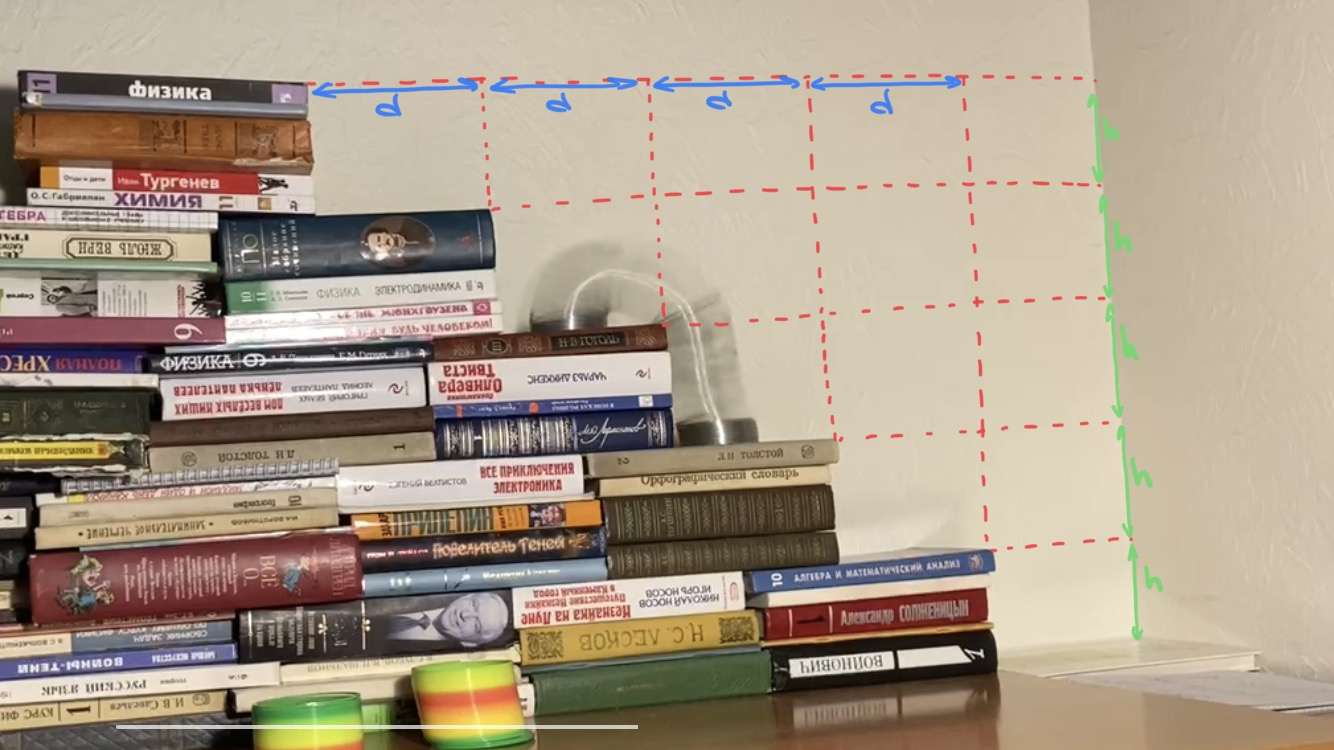
\includegraphics[scale=0.3]{установка.png}}
\caption{лабораторная установка}
\end{figure}

\begin{table}[H]
\centering
\scalebox{0.9}{
\begin{tabular}{|c|c|c|c|c|}
\hline
\multicolumn{5}{|c|}{\text{параметры   пружин}}                                                  \\ \hline
высота {[}см{]} & диаметр {[}см{]} & количество витков & длина растянутой {[}см{]} & масса {[}г{]} \\ \hline
\multicolumn{5}{|c|}{\text{короткая пластиковая}}                                                \\ \hline
4.4             & 7.5              & 28                & 58                        & 34            \\ \hline
\multicolumn{5}{|c|}{\text{длинная пластиковая}}                                                 \\ \hline
5.5             & 7.5              & 34                & 75                        & 45            \\ \hline
\multicolumn{5}{|c|}{\text{металлическая}}                                                       \\ \hline
6               & 6.8              & 80                & 115                       & 207           \\ \hline
\end{tabular}
}
\caption{параметры пружин}
\end{table}

Рассмотрим короткую пластиковую пружинку. Формула $\ref{period}$ показывает, что она делает один шаг за время $344\cdot10^{-3}с$ - сравним это время с экспериментальными данными из таблицы 2. Видим, что теретическое значение можно считать верным, так как оно содержится в доверительном интервале экспериментальных. При этом важно заметить, что при бОльшей ширине пружина не успевает перевалиться, а при меньшей перелетает. То есть мы сталкиваемся с границами применимости формулы $\ref{period}$. 

\begin{table}[H]
\centering
\begin{tabular}{|c|c|c|l|}
\hline
\text{\begin{tabular}[c]{@{}c@{}}высота\\      ступени {[}см{]}\end{tabular}} & \text{\begin{tabular}[c]{@{}c@{}}ширина\\      ступени {[}см{]}\end{tabular}} & \multicolumn{2}{c|}{\text{период {[}c{]}}}  \\ \hline
10                                                                              & 10                                                                              & \multicolumn{2}{c|}{$(363\pm23)\cdot10^{-3}$} \\ \hline
6                                                                               & 10                                                                              & \multicolumn{2}{c|}{$(361\pm18)\cdot10^{-3}$} \\ \hline
3                                                                               & 10                                                                              & \multicolumn{2}{c|}{$(355\pm19)\cdot10^{-3}$} \\ \hline
\end{tabular}
\caption{результаты экспериментов для короткой пластиковой пружинки.}
\end{table} 

Рассмотрим теперь длинную пластиковую пружинку. Формула $\ref{period}$ предсказывает время $391\cdot10^{-3}c$ - сравним это время с экспериментальными данными из таблицы 3. Как видно, здесь теория также оказывается верной. Но с поправкой на то, что пружина шагает: при иных параметрах лестницы она начинает слетать или застревает.

\begin{table}[H]
\centering
\begin{tabular}{|c|c|c|l|}
\hline
\begin{tabular}[c]{@{}c@{}}высота\\      ступени (см)\end{tabular} & \begin{tabular}[c]{@{}c@{}}ширина\\      ступени (см)\end{tabular} & \multicolumn{2}{c|}{период (c)}               \\ \hline
10                                                                 & 10                                                                 & \multicolumn{2}{c|}{$(424\pm18)\cdot10^{-3}$} \\ \hline
6                                                                  & 10                                                                 & \multicolumn{2}{c|}{$(418\pm18)\cdot10^{-3}$} \\ \hline
10                                                                 & 14                                                                 & \multicolumn{2}{c|}{$(424\pm22)\cdot10^{-3}$} \\ \hline
\end{tabular}
\caption{результаты экспериментов для длинной пластиковой пружинки.}
\end{table}

\textbf{ }
\\
\textbf{ }

Рассмотрим металлическую пружинку. Теоретически, время шага будет $484\cdot10^{-3}c$. Сравним с экспериментальными данными из таблицы 4. Здесь также становится ясно, что теория верна. Однако эта игрушка ходит только по строго подобранной лестнице.

\begin{table}[H]
\centering
\begin{tabular}{|c|c|c|l|}
\hline
\begin{tabular}[c]{@{}c@{}}высота\\      ступени (см)\end{tabular} & \begin{tabular}[c]{@{}c@{}}ширина\\      ступени (см)\end{tabular} & \multicolumn{2}{c|}{период (c)}               \\ \hline
6                                                                  & 10                                                                 & \multicolumn{2}{c|}{$(516\pm29)\cdot10^{-3}$} \\ \hline
10                                                                 & 14                                                                 & \multicolumn{2}{c|}{$(535\pm23)\cdot10^{-3}$} \\ \hline
\end{tabular}
\caption{результаты экспериментов для металлической пружинки.}
\end{table}

\subsection*{Падение} \text{ }
\addcontentsline{toc}{subsection}{Падение}

Закрепим пружину за верхний конец в вертикальной плоскости и посмотрим на её падение. Зафиксируем этот процесс на камеру, после чего на видео отследим положения концов и центра масс.

На раскадровке (рис.2) красным обозначается точка верхнего конца пружины, зеленым - середина, синим - нижний конец. Как видно, синяя точка стоит на месте до тех пор, пока верхняя не сократит расстояние между ними до высоты нерастянутой пружины. На приведенных кадрах пружина немного отклонилась от вертикали, так как способ запуска несовершенен. 

\begin{figure}[H]
\center{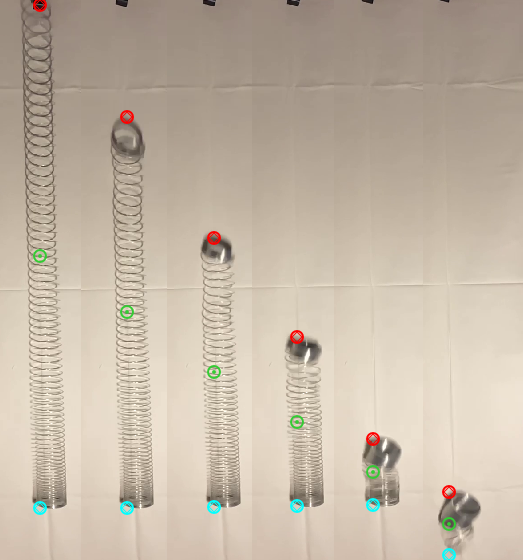
\includegraphics[scale=0.54]{динамика.png}}
\caption{Покадровое падение пружины}
\end{figure}

Эти же данные но в формате графика приведены на рисунке 3. Они позволяют увидеть, что хоть пружина и не в исходном состоянии, расстояние между точками все равно остается постоянным и равным её высоте.

\begin{figure} [H]
\center{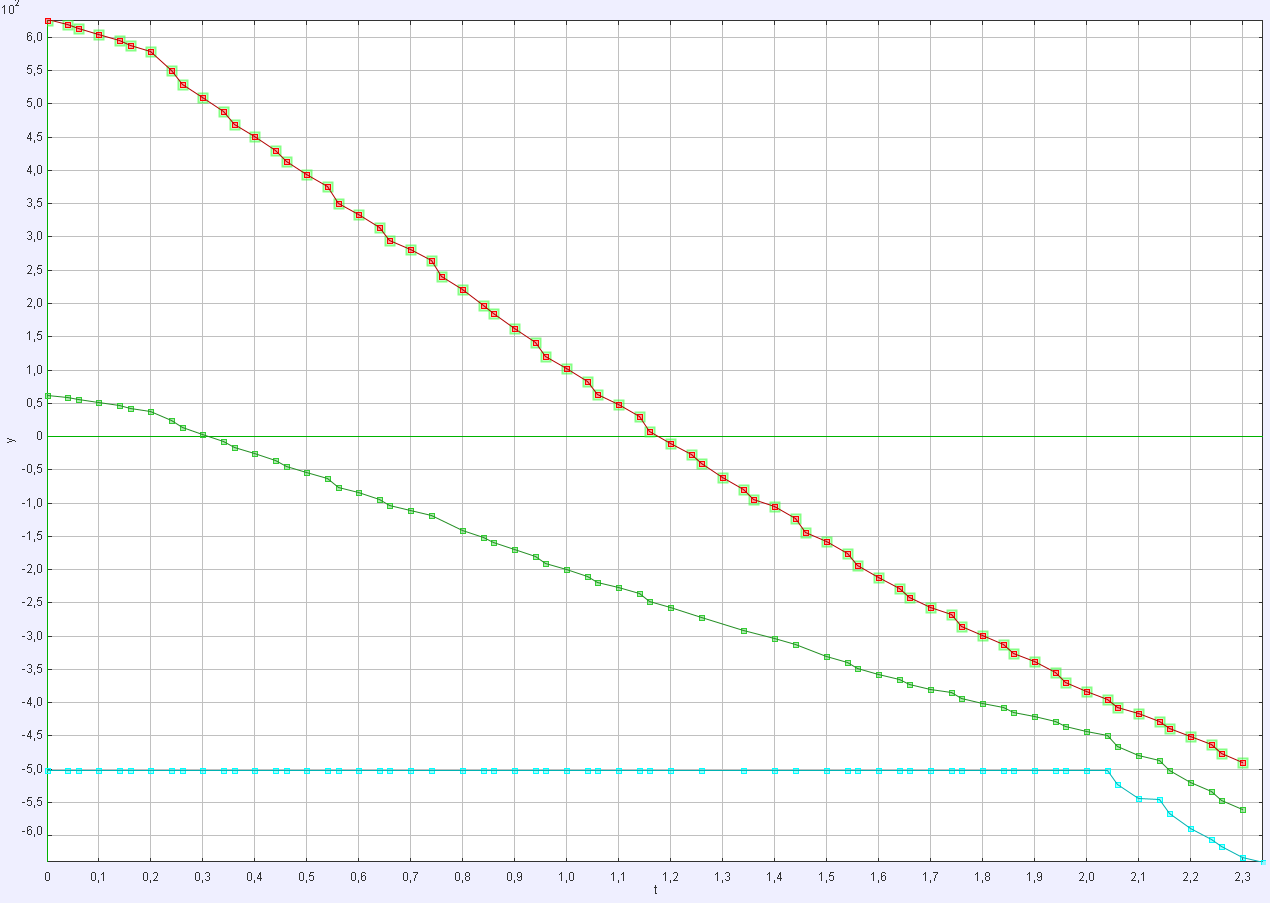
\includegraphics[scale=0.3]{графики.png}}
\caption{зависимость координаты от времени; зеленый - середина, голубой - нижний конец, красный - верхний конец.}
\end{figure}

\section*{Вывод} \text{ }
\addcontentsline{toc}{section}{Вывод}

Получили, что формула $\ref{period}$ действительно справедлива. То есть время спуска зависит только от параметров конкретной пружины. При этом у формул нет границ применимости, но есть условия спуска пружины. Получить их экспериментально не вышло, так как не позволило оборудование. В итоге пружина будет двигаться согласно выведенной формуле только тогда, когда её спуск будет представлять собой $"$правильные шаги$"$.

Из результатов наблюдения за падением следует, что этот неочевидный процесс на самом деле состоит из двух стадий. Верхняя часть пружины падает до уровня нижнего конца, при этом нижняя часть стоит на месте. После их встречи пружина падает как целое тело. При этом центр масс двигается как материальная точка, падающая с центра пружины. 



\end{document}
